%%%%%%%%%%%%%%%%%%%%%%%%%%%%%%%%%
% baposter Landscape Poster
% LaTeX Template
% Version 1.0 (15/5/13)
%
% Created by:
% Brian Amberg (baposter@brian-amberg.de)
%
% This template has been downloaded from:
% http://www.LaTeXTemplates.com
%
% License:
% CC BY-NC-SA 3.0 (http://creativecommons.org/licenses/by-nc-sa/3.0/)
%
%%%%%%%%%%%%%%%%%%%%%%%%%%%%%%%%%%%%%%%%%

%----------------------------------------------------------------------------------------
%	PACKAGES AND OTHER DOCUMENT CONFIGURATIONS
%----------------------------------------------------------------------------------------

\documentclass[a0paper,portrait,fontscale=0.35, margin=2cm]{baposter}

\usepackage[utf8]{inputenc}
\usepackage[font=normalsize,labelfont=bf]{caption} % Required for specifying captions to tables and figures
\captionsetup{justification=centering}
\usepackage{booktabs} % Horizontal rules in tables
\usepackage{lmodern}
\usepackage{relsize} % Used for making text smaller in some places

% Other packages
\usepackage{tabularx}
\def\tabularxcolumn#1{m{#1}}
\def\imagetop#1{\vtop{\null\hbox{#1}}}
\usepackage{adjustbox}
\usepackage{subfig}
\usepackage{floatrow} % sidecapfloat
\usepackage{setspace}
\usepackage{xspace}
\usepackage{noReferences}
\usepackage{caption}
\usepackage{tikz}
\usepackage[customcolors]{hf-tikz}
%\usepackage{subcaption}
\usepackage{epsf}
\usepackage{amsmath}
\usepackage{mathtools}
\usepackage{amssymb}
\usepackage{amsfonts}
\usepackage{amsthm}
\usepackage{dsfont}
\usepackage{enumitem}
\usepackage{float}
\usepackage{cases}
\usepackage{verbatim}
\usepackage{array}
\usepackage{graphicx}
\usepackage{graphics}
\usepackage{multirow}
\usepackage{listings}
%\usepackage[authoryear]{natbib}
\usepackage{authblk}
\usepackage[linesnumbered,ruled,vlined]{algorithm2e}
\usepackage{eqparbox}
\usepackage{xcolor}
\usepackage[backend=biber, citestyle=authoryear, maxcitenames=2, maxbibnames=2]{biblatex}
\usepackage{lipsum}
\usepackage{svg}

\bibliography{../references.bib}


% Colors for slides
\definecolor{rouge1}{RGB}{226,0,38}  % red P
\definecolor{orange1}{RGB}{243,154,38}  % orange P
\definecolor{jaune}{RGB}{254,205,27}  % jaune P
\definecolor{blanc}{RGB}{255,255,255} % blanc P

\definecolor{rouge2}{RGB}{230,68,57}  % red S
\definecolor{orange2}{RGB}{236,117,40}  % orange S
\definecolor{taupe}{RGB}{134,113,127} % taupe S
\definecolor{gris}{RGB}{91,94,111} % gris S
\definecolor{bleu1}{RGB}{38,109,131} % bleu S
\definecolor{bleu2}{RGB}{28,50,114} % bleu S
\definecolor{vert1}{RGB}{133,146,66} % vert S
\definecolor{vert3}{RGB}{20,200,66} % vert S
\definecolor{vert2}{RGB}{157,193,7} % vert S
\definecolor{vertsolarized}{RGB}{211,233,219} % vert S
\definecolor{darkyellow}{RGB}{233,165,0}  % orange S
\definecolor{lightgray}{rgb}{0.9,0.9,0.9}
\definecolor{darkgray}{rgb}{0.6,0.6,0.6}

\newcommand{\incarrow}{{
\includegraphics[height=0.7\baselineskip]{./img/arrow_list}}}


% Highlights for slides
\newcommand{\rcol}[1]{\textcolor{red}{\textit{#1}}}
%\newcommand{\eqrcol}[1]{\textcolor{red}{#1}}
%\newcommand{\eqrcolb}[1]{\textcolor{red}{\boldsymbol{#1}}}
\newcommand{\gcol}[1]{\textcolor{vert3}{\textit{#1}}}
%\newcommand{\eqgcol}[1]{\textcolor{vert3}{#1}}
%\newcommand{\eqgcolb}[1]{\textcolor{vert3}{\boldsymbol{#1}}}
\newcommand{\blcol}[1]{\textcolor{blue}{\textit{#1}}}
%\newcommand{\eqbcol}[1]{\textcolor{blue}{#1}}
%\newcommand{\eqbcolb}[1]{\textcolor{blue}{\boldsymbol{#1}}}
\newcommand{\ycol}[1]{\textcolor{darkyellow}{\textit{#1}}}
\newcommand{\eqycol}[1]{\textcolor{darkyellow}{#1}}

\newcommand{\rcolbm}[1]{$\textcolor{red}{\boldsymbol{#1}}$}
\newcommand{\rcolb}[1]{\textcolor{red}{\textit{\textbf{#1}}}}
\newcommand{\gcolb}[1]{\textcolor{vert3}{\textit{\textbf{#1}}}}
\newcommand{\bcolb}[1]{\textcolor{blue}{\textit{\textbf{#1}}}}
\newcommand{\ycolb}[1]{\textcolor{darkyellow}{\textit{\textbf{#1}}}}

% Colored boxes
\newcounter{ColoredBoxesCounter}
\newcommand{\highlightnew}[3][(0.0,-0.1)(-0.0,0.3)]{
\hfsetfillcolor{#2!20}
\hfsetbordercolor{#2!80}
\tikzmarkin{\theColoredBoxesCounter}#1
#3
\tikzmarkend{\theColoredBoxesCounter}
\stepcounter{ColoredBoxesCounter}
}

\newcommand{\highlight}[2][yellow]{\mathchoice%
{\colorbox{#1}{$\displaystyle#2$}}%
{\colorbox{#1}{$\textstyle#2$}}%
{\colorbox{#1}{$\scriptstyle#2$}}%
{\colorbox{#1}{$\scriptscriptstyle#2$}}}%

\newcommand{\eqrcol}[1]{\highlight[red!20]{#1}}
\newcommand{\eqrcolb}[1]{\highlight[red!20]{\boldsymbol{#1}}}
\newcommand{\eqgcol}[1]{\highlight[vert3!20]{#1}}
\newcommand{\eqgcolb}[1]{\highlight[vert3!20]{\boldsymbol{#1}}}
\newcommand{\eqbcol}[1]{\highlight[blue!20]{#1}}
\newcommand{\eqbcolb}[1]{\highlight[blue!20]{\boldsymbol{#1}}}

\colorlet{redp}{red!20} % vert S
\colorlet{greenp}{vert3!20} % vert S
\colorlet{bluep}{blue!20} % vert S
\colorlet{yellowp}{yellow!20} % vert S

\renewcommand{\hl}[3][\fboxsep1pt]{{#1\colorbox{#2}{#3}}}%

\newcommand{\hlr}[1]{\hl{redp}{#1}}
\newcommand{\hlg}[1]{\hl{greenp}{#1}}
\newcommand{\hlb}[1]{\hl{bluep}{#1}}
\newcommand{\hly}[1]{\hl{yellowp}{#1}}

\newcommand{\hler}[1]{\hl[\fboxsep0pt]{redp}{$\displaystyle {#1}$}}
\newcommand{\hleg}[1]{\hl[\fboxsep0pt]{greenp}{$\displaystyle {#1}$}}
\newcommand{\hleb}[1]{\hl[\fboxsep0pt]{bluep}{$\displaystyle {#1}$}}

\newcommand{\hlbr}[1]{\hl[\fboxsep0pt]{redp}{$\displaystyle \mathbf{#1}$}}
\newcommand{\hlbg}[1]{\hl[\fboxsep0pt]{greenp}{$\displaystyle \mathbf{#1}$}}
\newcommand{\hlbb}[1]{\hl[\fboxsep0pt]{bluep}{$\displaystyle \mathbf{#1}$}}

\newcommand{\vph}{\vphantom{A_A^A}}

% Box for algorithms
\newlength{\minipagewidth}
\newlength{\minipagewidthx}
\setlength{\minipagewidth}{\columnwidth}
\setlength{\minipagewidthx}{\columnwidth}
\setlength{\fboxsep}{0.1mm}
\addtolength{\minipagewidth}{-\fboxrule}
\addtolength{\minipagewidth}{-\fboxrule}
\addtolength{\minipagewidth}{-\fboxsep}
\addtolength{\minipagewidth}{-\fboxsep}
\addtolength{\minipagewidthx}{+\fboxsep}
\newcommand{\bookbox}[1]{\small
\par\medskip\noindent
\framebox[\columnwidth]{
\begin{minipage}{\minipagewidth} {#1} \end{minipage} } \par\medskip }

\newcommand{\bookboxx}[1]{
\par\medskip\noindent
\framebox[\columnwidth]{
\begin{minipage}[t]{0.98\columnwidth} {\par\smallskip#1\par\smallskip} \end{minipage} } \par\medskip }


\usepackage{array}
\newcolumntype{L}[1]{>{\raggedright\let\newline\\\arraybackslash\hspace{-3.1cm}}m{#1}}
\newcolumntype{C}[1]{>{\centering\let\newline\\\arraybackslash\hspace{135pt}}m{#1}}
\newcolumntype{R}[1]{>{\raggedleft\let\newline\\\arraybackslash\hspace{-10pt}}m{#1}}

\newenvironment{myfont}{\fontfamily{kurier}\selectfont}{\par}
\newenvironment{myfont2}{\fontfamily{epigrafica}\selectfont}{\par}

% Border color of content boxes
\definecolor{bordercol}{RGB}{0,0,0}  %black
% Background color for the header in the content boxes (left side)
\definecolor{headercol1}{RGB}{200,0,0}        %red:RGB {200,0,0} 
% Background color for the header in the content boxes (right side) 
\definecolor{headercol2}{rgb}{1.0,0.49,0.0}        %orange:rgb {1.0,0.49,0.0}
% Text color for the header text in the content boxes
\definecolor{headerfontcol}{rgb}{1,1,1}  %white
% Background color for the content in the boxes
\definecolor{boxcolor}{rgb}{1,1,1} 

\definecolor{lightblue}{rgb}{0.145,0.6666,1}

\newsavebox\CBox
\newcommand\hcancel[2][0.5pt]{%
  \ifmmode\sbox\CBox{$#2$}\else\sbox\CBox{#2}\fi%
  \makebox[0pt][l]{\usebox\CBox}%  
  \rule[0.3\ht\CBox-#1/2]{\wd\CBox}{#1}}



%%%%%%%%%%%%%%%%%%%%%%%%%%%%
% Paper dependent stuff    %
%%%%%%%%%%%%%%%%%%%%%%%%%%%%

\newcommand{\Tau}{\mathcal{T}}
\newcommand{\LL}{\mathcal{L}}
\newcommand{\dquad}{d_\texttt{QUAD}}
\newcommand{\dber}{d_\texttt{BER}}
\newcommand{\OLOP}{\texttt{OLOP}\xspace}
\newcommand{\ODP}{\texttt{ODP}\xspace}
\newcommand{\KLOLOP}{\texttt{KL-OLOP}\xspace}
\newcommand{\klOLOP}{\texttt{kl-OLOP}\xspace}


%%%%%%%%%%%%%%%%%%%%%%%%%%%%
% Aesthetics               %
% over-underline, hat, bold%
%%%%%%%%%%%%%%%%%%%%%%%%%%%%

%%% miso
\newcommand{\eps}{\varepsilon}
\newcommand{\vareps}{\varepsilon}
\renewcommand{\epsilon}{\varepsilon}
%\renewcommand{\hat}{\widehat}
\renewcommand{\tilde}{\widetilde}
\renewcommand{\bar}{\overline}

\newcommand*{\MyDef}{\mathrm{\tiny def}}
\newcommand*{\eqdefU}{\ensuremath{\mathop{\overset{\MyDef}{=}}}}% Unscaled version
%\newcommand*{\eqdef}{\mathop{\overset{\MyDef}{\resizebox{\widthof{\eqdefU}}{\heightof{=}}{=}}}}


\def\:#1{\protect \ifmmode {\mathbf{#1}} \else {\textbf{#1}} \fi}
\newcommand{\CommaBin}{\mathbin{\raisebox{0.5ex}{,}}}

\newcommand{\wt}[1]{\widetilde{#1}}
\newcommand{\wh}[1]{\widehat{#1}}
\newcommand{\wo}[1]{\overline{#1}}
\newcommand{\wb}[1]{\overline{#1}}

% bf and bm missing due to conflict!!
\newcommand{\bsym}[1]{\mathbf{#1}}
\newcommand{\bzero}{\mathbf{0}}
\newcommand{\ba}{\mathbf{a}}
\newcommand{\bb}{\mathbf{b}}
\newcommand{\bc}{\mathbf{c}}
\newcommand{\bd}{\mathbf{d}}
\newcommand{\be}{\mathbf{e}}
\newcommand{\bg}{\mathbf{g}}
\newcommand{\bh}{\mathbf{h}}
\newcommand{\bi}{\mathbf{i}}
\newcommand{\bj}{\mathbf{j}}
\newcommand{\bk}{\mathbf{k}}
\newcommand{\bl}{\mathbf{l}}
\newcommand{\bn}{\mathbf{n}}
\newcommand{\bo}{\mathbf{o}}
\newcommand{\bp}{\mathbf{p}}
\newcommand{\bq}{\mathbf{q}}
\newcommand{\br}{\mathbf{r}}
\newcommand{\bs}{\mathbf{s}}
\newcommand{\bt}{\mathbf{t}}
\newcommand{\bu}{\mathbf{u}}
\newcommand{\bv}{\mathbf{v}}
\newcommand{\bw}{\mathbf{w}}
\newcommand{\bx}{\mathbf{x}}
\newcommand{\by}{\mathbf{y}}
\newcommand{\bz}{\mathbf{z}}

\newcommand{\bA}{\mathbf{A}}
\newcommand{\bB}{\mathbf{B}}
\newcommand{\bC}{\mathbf{C}}
\newcommand{\bD}{\mathbf{D}}
\newcommand{\bE}{\mathbf{E}}
\newcommand{\bF}{\mathbf{F}}
\newcommand{\bG}{\mathbf{G}}
\newcommand{\bH}{\mathbf{H}}
\newcommand{\bI}{\mathbf{I}}
\newcommand{\bJ}{\mathbf{J}}
\newcommand{\bK}{\mathbf{K}}
\newcommand{\bL}{\mathbf{L}}
\newcommand{\bM}{\mathbf{M}}
\newcommand{\bN}{\mathbf{N}}
\newcommand{\bO}{\mathbf{O}}
\newcommand{\bP}{\mathbf{P}}
\newcommand{\bQ}{\mathbf{Q}}
\newcommand{\bR}{\mathbf{R}}
\newcommand{\bS}{\mathbf{S}}
\newcommand{\bT}{\mathbf{T}}
\newcommand{\bU}{\mathbf{U}}
\newcommand{\bV}{\mathbf{V}}
\newcommand{\bW}{\mathbf{W}}
\newcommand{\bX}{\mathbf{X}}
\newcommand{\bY}{\mathbf{Y}}
\newcommand{\bZ}{\mathbf{Z}}

% calligraphic
\newcommand{\cf}{\mathcal{f}}
\newcommand{\cA}{\mathcal{A}}
\newcommand{\cB}{\mathcal{B}}
\newcommand{\cC}{\mathcal{C}}
\newcommand{\cD}{\mathcal{D}}
\newcommand{\cE}{\mathcal{E}}
\newcommand{\cF}{\mathcal{F}}
\newcommand{\cG}{\mathcal{G}}
\newcommand{\cH}{\mathcal{H}}
\newcommand{\cI}{\mathcal{I}}
\newcommand{\cJ}{\mathcal{J}}
\newcommand{\cK}{\mathcal{K}}
\newcommand{\cL}{\mathcal{L}}
\newcommand{\cM}{\mathcal{M}}
\newcommand{\cN}{\mathcal{N}}
\newcommand{\cO}{\mathcal{O}}
\newcommand{\cP}{\mathcal{P}}
\newcommand{\cQ}{\mathcal{Q}}
\newcommand{\cR}{\mathcal{R}}
\newcommand{\cS}{\mathcal{S}}
\newcommand{\cT}{\mathcal{T}}
\newcommand{\cU}{\mathcal{U}}
\newcommand{\cV}{\mathcal{V}}
\newcommand{\cW}{\mathcal{W}}
\newcommand{\cX}{\mathcal{X}}
\newcommand{\cY}{\mathcal{Y}}
\newcommand{\cZ}{\mathcal{Z}}

%%%%%%%%%%%%%%%%%%%%%%%%%%%%
% Math jargon              %
%%%%%%%%%%%%%%%%%%%%%%%%%%%%
\newcommand{\wrt}{w.r.t.\xspace}
\newcommand{\defeq}{\stackrel{\mathclap{\normalfont\mbox{\tiny def}}}{=}}
\newcommand{\maxund}[1]{\max\limits_{#1}}
\newcommand{\supund}[1]{\text{sup}\limits_{#1}}
\newcommand{\minund}[1]{\min\limits_{#1}}
\renewcommand{\epsilon}{\varepsilon}
\newcommand{\bigotime}{\mathcal{O}}


\DeclareMathOperator*{\argmin}{arg\,min} 
\DeclareMathOperator*{\argmax}{arg\,max} 
\DeclareMathOperator*{\cupdot}{\mathbin{\mathaccent\cdot\cup}}
\newcommand{\eqdef}{\buildrel \text{def}\over =}

%%%%%%%%%%%%%%%%%%%%%%%%%%%%
% Matrix operators         %
%%%%%%%%%%%%%%%%%%%%%%%%%%%%
\newcommand{\transpose}{^\mathsf{\scriptscriptstyle T}}
\newcommand{\transp}{\mathsf{\scriptscriptstyle T}}

%%%%%%%%%%%%%%%%%%%%%%%%%%%%
% Statistic operators      %
%%%%%%%%%%%%%%%%%%%%%%%%%%%%
\newcommand{\probability}[1]{\mathbb{P}\left(#1\right)}
\newcommand{\probdist}{Pr}
\DeclareMathOperator*{\expectedvalue}{\mathbb{E}}
\DeclareMathOperator*{\variance}{\text{Var}}
\newcommand{\expectedvalueover}[1]{\expectedvalue\limits_{#1}}
\newcommand{\condbar}{\;\middle|\;}
\newcommand{\gaussdistr}{\mathcal{N}}
\newcommand{\uniformdistr}{\mathcal{U}}
\newcommand{\bernoullidist}{\mathcal{B}}

%%%%%%%%%%%%%%%%%%%%%%%%%%%%
% Algebraic Sets           %
%%%%%%%%%%%%%%%%%%%%%%%%%%%%
\newcommand{\Real}{\mathbb{R}}
\newcommand{\Natural}{\mathbb{N}}
\newcommand{\statespace}{\mathcal{X}}
\newcommand{\funcspace}{\mathcal{F}}
\newcommand{\dynaspace}{\mathcal{T}}


% \newtheorem{theorem}{Theorem}
% \newtheorem{definition}{Definition}
% \newtheorem{lemma}{Lemma}
\newtheorem{proposition}{Proposition}
\newtheorem{assumption}{Assumption}
\newtheorem{remark}{Remark}
\newtheorem{property}{Property}

% Removed from mathdef because of conflict with paper lcns class
\newtheorem{theorem}{Theorem}
\newtheorem{definition}{Definition}
\newtheorem{lemma}{Lemma}
\newtheorem{proposition}{Proposition}
\newtheorem{remark}{Remark}
\newtheorem{property}{Property}

\begin{document}


%\background{ % Set the background to an image (background.pdf)
%\begin{tikzpicture}[remember picture,overlay]
%\draw (current page.north west)+(-2em,2em) node[anchor=north west]
%{\includegraphics[height=1.1\textheight]{background.png}};
%\end{tikzpicture}
%}
\begin{poster}{
grid=false,
borderColor=bordercol, % Border color of content boxes
headerColorOne=headercol1, % Background color for the header in the content boxes (left side)
headerColorTwo=headercol2, % Background color for the header in the content boxes (right side)
headerFontColor=headerfontcol, % Text color for the header text in the content boxes
boxColorOne=boxcolor, % Background color for the content in the content boxes
headershape=roundedright, % Specify the rounded corner in the content box headers
%headerfont=\Large\sf\bf, % Font modifiers for the text in the content box headers
headerfont=\Large\bf\textsc, %Sans Serif
textborder=rectangle,
background=none,
headerborder=open, % Change to closed for a line under the content box headers
boxshade=plain,
textfont={\setlength{\parindent}{0.0em}\sffamily},
headerheight={0.05\textheight},
eyecatcher=true
%columns=5
}
%
%----------------------------------------------------------------------------------------
%	Title and authors
%----------------------------------------------------------------------------------------
%
{

\includegraphics[width=14em]{./img/renault_group}
}
{
Practical Open-Loop Optimistic Planning
}
{
Edouard Leurent, Odalric-Ambrym Maillard
\vspace{-4\baselineskip}
}
{

\includegraphics[width=14em]{./img/inria_sc}
}

\setlength{\colheight}{0.92\textheight}

%----------------------------------------------------------------------------------------
%	Motivation
%----------------------------------------------------------------------------------------

\headerbox{\textsc{Motivation}}{name=motivation,span=1,column=0,row=0}{

We consider the optimal control of an MDP $\cM = (\cS, A, R, T, \gamma)$ with bounded rewards $R\in[0,1]$
\begin{itemize}[nolistsep]
    \item[\incarrow] $R$ and $T$ are \hlr{unknown}
    \item[\incarrow] Access to a \hlb{generative model} $s' \sim \probability{s'|s,a}$ and $r\sim\probability{r|s, a}$
    \item[\incarrow] \hlr{Fixed-budget} setting: the generative model is \hlr{costly}, can only be queried $n$ times
\end{itemize}
}

%----------------------------------------------------------------------------------------
%	Setting
%----------------------------------------------------------------------------------------
\headerbox{\textsc{Open-Loop Optimistic Planning}}{name=setting,span=1,column=0,row=0,below=motivation}{
\OLOP algorithm introduced in [\cite{Bubeck2010}].


%Split the budget $n$ into $M$ sequences of length $L$.
%Let $M$ be the largest integer such that $M \log M/(2 \log 1/\gamma) \leq n$\;
%Let $L = \log M / (2 \log 1/\gamma)$\;
\begin{enumerate}
    \item Sample $M$ sequences of actions of fixed length $L$
    \begin{center}
\includesvg[width=0.8\textwidth]{img/olop-explain.svg}
\end{center}
    \item Use the \hlb{return structure} to \hlb{generalise} to unseen sequences
    \begin{center}
\includesvg[width=0.8\textwidth]{img/olop-explain-2.svg}
\end{center}
\item Be \hlb{Optimistic in the Face of Uncertainty}\\
    \incarrow~ in \hlr{observed} and \hlr{future} rewards
\end{enumerate}

\begin{center}
\begin{algorithm}[H]
\DontPrintSemicolon
\footnotesize
\For{each episode $m = 1, \cdots, M$}{
Compute $U_a(m-1)$ from \eqref{eq:Ua} for all $a\in\mathcal{T}$\;
Compute $B_a(m-1)$ from \eqref{eq:Ba} for all $a\in A^L$\;\label{alg:b_values_compute}
Sample a sequence with highest B-value: $a^m \in \argmax_{a\in A^L} B_a(m-1)$.\;
}
\Return the most played sequence $a(n) \in \argmax_{a\in A^L} T_a(M)$
\caption{General structure for Open-Loop Optimistic Planning}
\label{algo:kl-olop}
\end{algorithm}
\end{center}

}

%----------------------------------------------------------------------------------------
% Tools
%----------------------------------------------------------------------------------------
\headerbox{\textsc{What's wrong with OLOP?}}
{name=tools,column=0,below=setting,span =1}
{

\hlr{Overly pessimistic}, especially in the low-budget regime.

\begin{equation}
         U^{\mu}_a(m) = \hat{\mu}_a(m) + \sqrt{\frac{2 \log M}{T_a(m)}}
    \end{equation}
    \begin{equation}
    \label{eq:Ua}
        U_a(m) \eqdef \sum_{t = 1}^h \gamma^t U^{\mu}_{a_{1:t}}(m) + \frac{\gamma^{h+1}}{1-\gamma}
    \end{equation}
    \begin{equation}
    \label{eq:Ba}
        B_a(m) \eqdef \inf_{1 \leq t \leq L} U_{a_{1:t}}(m)
    \end{equation}
    Intuitive explanation: 
    \begin{itemize}
        \item Unintended behaviour happens when $\hler{U^{\mu}_a(m) > 1}, \forall a$. 
        \item Then the sequence $(U_{a_{1:t}}(m))_t$ is non-decreasing
        \item Then \hlr{$B_a(m) = U_{a_{1:1}}(m)$}
    \end{itemize}

\begin{center}
\includesvg[width=0.8\textwidth]{img/olop-explain-3.svg}    
\end{center}

\begin{center}
\texttt{OLOP} behaves as \hlr{uniform planning}!    
\end{center}
}


%----------------------------------------------------------------------------------------
%	KL-OLOP
%----------------------------------------------------------------------------------------
\headerbox{\textsc{Kullback-Leibler OLOP}}{name=klolop,column=1,span=2}{

\begin{minipage}[]{0.59\textwidth}
 We summon the upper-confidence bound from \texttt{kl-UCB} [\cite{Cappe2013}]:
    \begin{equation*}
        U^{\mu}_a(m) \eqdef \max \left\{q\in I: d(\hat{\mu}_a(m), q) \leq \frac{f(m)}{T_a(m)} \right\}
    \end{equation*}
    
    \begin{center}
    \begin{tabular}{ccc}
    \toprule
        Algorithm & \texttt{OLOP} & \texttt{KL-OLOP} \\
        \midrule
        Interval $I$ & $\mathbb{R}$ & [0, 1] \\
        Divergence $d$ & $d_{\texttt{QUAD}}$ & $d_{\texttt{BER}}$ \\
        $f(m)$ & $4 \log M$ & $2\log M + 2 \log\log M$\\
        \bottomrule
    \end{tabular}
    \end{center}
    with
    \begin{align*}
    d_{\texttt{QUAD}}(p,q) &\eqdef 2(p-q)^2\\
    d_{\texttt{BER}}(p, q) &\eqdef p \log \frac{p}{q} + (1-p)\log\frac{1-p}{1-q}
    \end{align*}
\end{minipage}
\begin{minipage}[]{0.4\textwidth}
    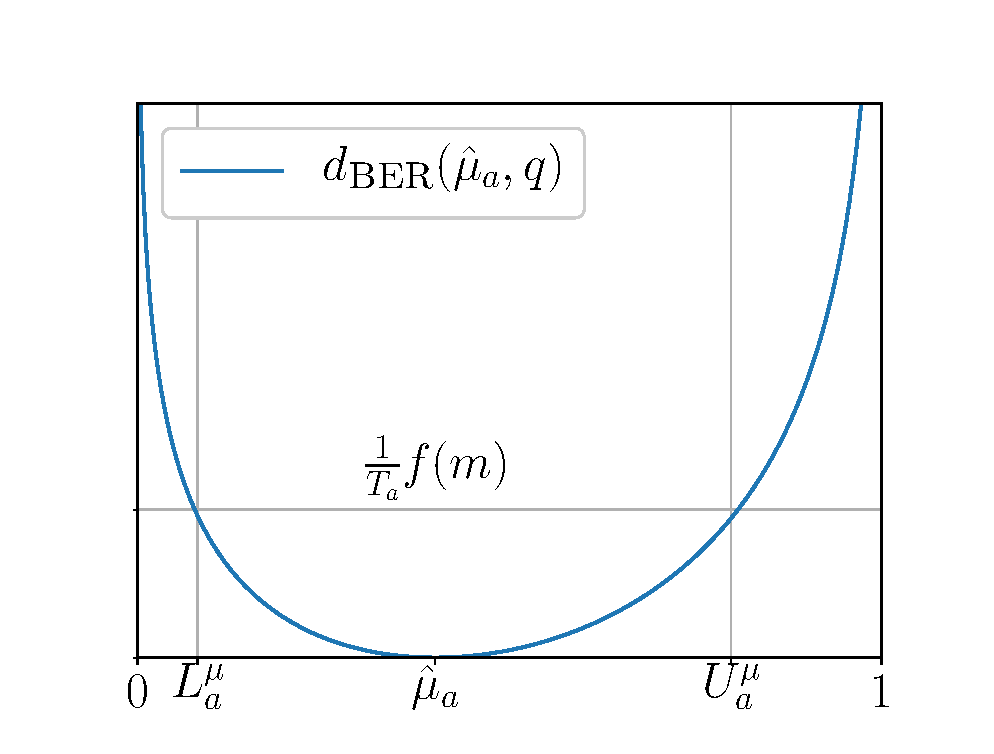
\includegraphics[width=\textwidth]{../img/ukl}
\end{minipage}
    
Conversely,
\begin{itemize}
    \item \hlg{$U^{\mu}_a(m) \in I = [0, 1], \forall a$}. 
    \item The sequence $(U_{a_{1:t}}(m))_t$ is \hlg{non-increasing}
    \item $B_a(m) = U_a(m)$, the \emph{bound sharpening} step is \hlb{superfluous}.
\end{itemize}
}

%----------------------------------------------------------------------------------------
%	Sample Complexity
%----------------------------------------------------------------------------------------
\headerbox{Sample complexity}{name=sample,span=2,column=1,below=klolop}{ 
\begin{theorem}[Sample complexity]
\label{thm:regret}
\KLOLOP enjoys the same asymptotic regret bounds as \OLOP. More precisely, \KLOLOP satisfies:
\begin{equation*}
    \expectedvalue r_n = \begin{cases}
      \tilde{0}\left(n^{-\frac{\log 1/\gamma}{\log \kappa'}}\right), & \text{if}\ \gamma\sqrt{\kappa'} > 1 \\
      \tilde{0}\left(n^{-\frac{1}{2}}\right), & \text{if}\ \gamma\sqrt{\kappa'} \leq 1
    \end{cases}
\end{equation*}
\end{theorem}
}

%----------------------------------------------------------------------------------------
%	Time and Memory Complexity
%----------------------------------------------------------------------------------------
\headerbox{Time and memory complexity}{name=time,span=2,column=1,below=sample}{ 

\begin{tabular}{>{\centering}p{0.45\textwidth}>{\centering}p{0.5\textwidth}}
\begin{minipage}[]{0.45\textwidth}

\textbf{Original \KLOLOP}

\emph{Compute $B_a(m-1)$ from \eqref{eq:Ba} \hlr{for all $a\in A^L$}}

\textbf{Lazy \KLOLOP}
\begin{center}
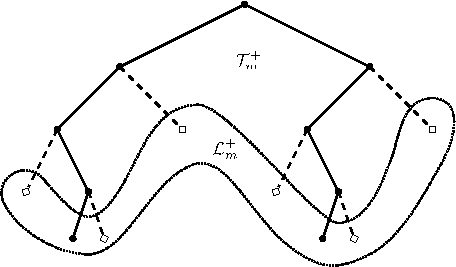
\includegraphics[width=0.8\textwidth]{../img/tree_svg-tex}    
\end{center}

\begin{theorem}[Consistency]
\label{thm:consistency}
Algorithm \ref{algo:lazy-kl-olop} is \hlg{identical} to Algorithm \ref{algo:kl-olop}.
\end{theorem}
\end{minipage}

&

\begin{minipage}{0.5\textwidth}
    \begin{algorithm}[H]
\DontPrintSemicolon
\footnotesize
Let $\Tau_0^+ = \LL_0^+ = \{\emptyset\}$\;
\For{each episode $m = 1, \cdots, M$}{
Compute $U_a(m-1)$ from \eqref{eq:Ua} for all \hlg{$a\in\Tau_{m-1}^+$}\;
Compute $B_a(m-1)$ from \eqref{eq:Ba} for all \hlg{$a\in \LL_{m-1}^+$}\;
Sample a sequence with highest B-value: $a \in \argmax_{\hleg{a\in \LL_{m-1}^+}} B_a(m-1)$\;
Choose an arbitrary continuation $a^m \in aA^{L-|a|}$\tcp*[h]{e.g. uniformly}
Let $\Tau_m^+ = \Tau_{m-1}^+$ and $\LL_m^+ = \LL_{m-1}^+$\;
\For{$t=1, \cdots, L$}{
    \If{$a^m_{1:t} \not \in \Tau_{m}^+$}{
    \hlb{Add $a^m_{1:t-1}A$ to $\Tau_{m}^+$ and $\LL_{m}^+$}\;
    \hlb{Remove $a^m_{1:t-1}$ from $\LL_{m}^+$}
    }
}
}
\Return the most played $a(n) \in \argmax_{a\in \LL_m^+} T_a(M)$
\caption{Lazy Open Loop Optimistic Planning}
\label{algo:lazy-kl-olop}
\end{algorithm}
\end{minipage}
\end{tabular}

\begin{property}[Time and memory complexity]
\begin{equation*}
    \frac{C(\texttt{Lazy KL-OLOP})}{C(\texttt{KL-OLOP})} = \frac{\hleg{nA}}{\hler{A^{L}}}
\end{equation*}
\end{property}

}

%
%%----------------------------------------------------------------------------------------
%% Experiments
%%----------------------------------------------------------------------------------------
%
\headerbox{Experiments}{name=experiments,span=2,column=1,below=time, above=bottom}{ 
     \includesvg[width=0.33\textwidth]{../img/hw_return}
     \includesvg[width=0.33\textwidth]{../img/gw_return}
     \includesvg[width=0.33\textwidth]{../img/gw_stoch_return}
     \begin{center}
         \textbf{Average return} over 100 runs –- along with its 95\% confidence interval –- with respect to the available budget $n$
     \end{center}

    \includesvg[width=0.33\textwidth]{../img/tree-ODP}    \includesvg[width=0.33\textwidth]{../img/tree-OLOP}
    \includesvg[width=0.33\textwidth]{../img/tree-KL-OLOP}
    \begin{center}
        \textbf{Expanded trees} for a budget $n=10^3$
    \end{center}
}



%----------------------------------------------------------------------------------------
%	Acknowledgements
%----------------------------------------------------------------------------------------
% \headerbox{Acknowledgements}{name=ack,column=0,span=1,below=tools}{
% This work has been supported by CPER Nord-Pas de Calais/FEDER DATA Advanced data science and technologies 2015-2020, the French Ministry of Higher Education and Research, INRIA, and the French Agence Nationale de la Recherche (ANR).
% }


%----------------------------------------------------------------------------------------
%	References
%----------------------------------------------------------------------------------------
\headerbox{References}{name=refs,column=0,span=1,below=tools, above=bottom}{
    {
    \AtNextBibliography{\footnotesize}
    \setlength{\bibitemsep}{3pt}
    \printbibliography[heading=none]
    }
}


\end{poster}

\end{document}


